%% This LaTeX-file was created by <imt> Thu May  7 16:54:43 1998
%% LyX 0.12 (C) 1995-1998 by Matthias Ettrich and the LyX Team

%% Do not edit this file unless you know what you are doing.
\documentclass{article}
\usepackage[T1]{fontenc}
\usepackage{makeidx}
\makeindex
\usepackage{graphics}

\makeatletter


%%%%%%%%%%%%%%%%%%%%%%%%%%%%%% LyX specific LaTeX commands.
\newcommand{\LyX}{L\kern-.1667em\lower.25em\hbox{Y}\kern-.125emX\spacefactor1000}

\makeatother

\begin{document}


\title{Feasibility Study}


\author{System Design Group Seven }

\maketitle
\vspace{0.3cm}
{\centering 
\includegraphics{../web/images/EUcrest-official-noborder.ps} \par}
\vspace{0.3cm}

\newpage
\tableofcontents

\printindex


\newpage
\section{Introduction}

Ding Dong Door-entry Systems Ltd has commissioned our group to develop an idea
for a new product. Their business has so far been based on selling simple but
supposedly vandal proof door entry systems for stair doors. Their new idea involves
branching out into high specification door-entry systems, and in particular,
taking advantage of the fact that most small companies and many homes now have
a PC inside them. Since PC's already incorporate a screen and sound facilities,
the intention is to sell a door-entry system that allows a person within the
premises to use a PC to view the person at the door. This unit would be sold
together with the necessary PC software .

Since all PCs have serial ports, Ding Dong's idea is to produce a unit to be
sited by the door which interfaces to the PC via a serial port. This unit would
be sold together with the necessary PC software.

Ding Dong would also like to offer the facility of having the PC contol entry
automatically (ie without a person being present at the PC) and suggest this
could be done by operating the door with a combination of some kind of personal
card or key, and a PIN number.

We have been commissioned to produce, rapidly and inexpensively, a demonstration
prototype. We have have to refine their vague specification for the product,
decide on the best way to provide the facilities that Ding Dong wants to see,
and to develop additional features that might increase the product's marketability.


\newpage
\section{Market Research}

The design specification identified two markets for the product. We carried
out a survey to gauge the degree of practicality and interest in producing a
product for these markets. The results are separated into residential and commercial
Properties


\subsection{Residential Properties}

We carried out an informal survey of 127 residents in and around Marchmont.
The accommodation in this area mostly comprises of flats and the majority of
people are aged between 20-35 years old. They were all told the idea of the
product before the questions were asked. Anybody who answered no to any question,
was excluded from the rest of the survey.

\vspace{0.3cm}
{\centering \begin{tabular}{|c|c|c|}
\hline 
Residential&
YES&
NO\\
\hline 
\hline 
Do you have a PC in you Household?&
42&
85\\
\hline 
Do you have some form of door entry system?&
35&
7\\
\hline 
Would you be interested in combining the PC with a door entry system?&
6&
29\\
\hline 
\end{tabular}\par}
\vspace{0.3cm}

Our survey indicates that only 17\% of the people who had a PC and a door entry
system would be interested in a product that combined the two. Although the
market demand currently is low; the demand in future may rise. We identified
the main residential markets to assess their likely future demands.


\subsubsection{Blocks of Flats }

\vspace{0.3cm}
{\centering 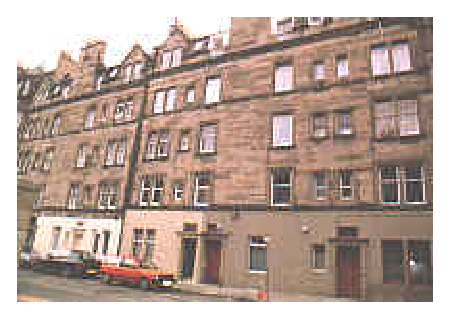
\includegraphics{../web/images/pw3375.ps} \par}
\vspace{0.3cm}

The increase of PC's in the home may allow this product to become an alternative
to the standard door-entry system. According to a representative of Castle Security
(a local security company) the system would face the problem of convincing sections
of the population of its value. There will always be a percentage who will be
resistant to new technology, and a section who will resist having to pay for
a new technology. 


\subsubsection{Accommodation with a servitor}

\vspace{0.3cm}
{\centering \resizebox*{6cm}{!}{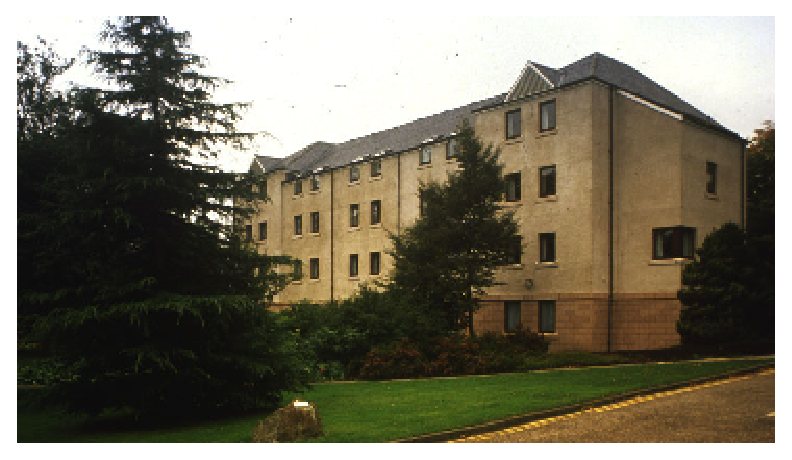
\includegraphics{../web/images/masson.ps}} \par}
\vspace{0.3cm}

The servitors office would contain the PC and during the day people could be
let in by visual identification only. During the night a form of security could
be set for the main entrances. The potential here is for accommodation similar
to halls of residence. 

A spokesman for Pollock halls of residence was enthusiastic about the system,
the individual halls all have offices next to the only entrance, all the offices
also contain PC's that are unused overnight. The system would be beneficial
in enabling only residents to enter their building after the site has been locked.
They also suggested an application for the front gate of the halls were they
use visual identification to let cars in. It would be cheaper to run the system
automatically than to hire doormen.


\subsubsection{Semi / Detached Property}

\vspace{0.3cm}
{\centering \resizebox*{8cm}{6cm}{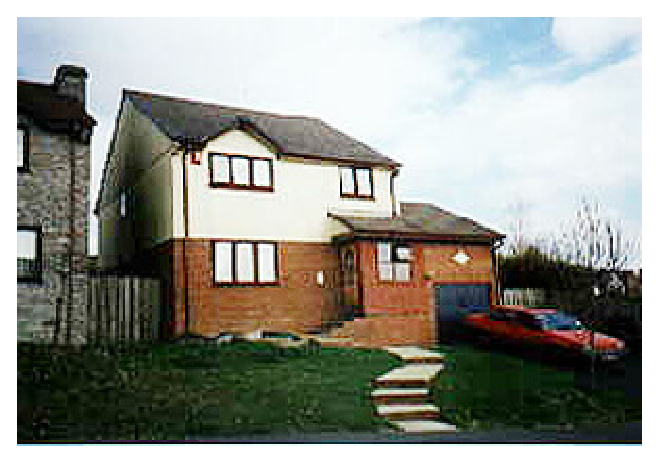
\includegraphics{../web/images/b2ivy163.ps}} \par}
\vspace{0.3cm}

Presently these properties have little or no door entry system; convincing them
to purchase an audio/visual system would mean convining them that they need
some form of access control. 

The biggest market in this area would be properties sited within large grounds
ie. estate houses which can have entrances that are set a significant distance
away from the property. These properties could use the improved security of
visual communication. 


\subsection{Conclusion}

Examining the residential user group; their needs and their response to our
proposed design it is clear that although there is enthusiasm from some parts
of the market (eg Pollock halls) most others currently have no need or desire
to own this product. The majority of people are quite happy with their present
system.


\subsection{Commercial}


\subsubsection{Small/Large Business}

We carried out an informal survey of fourteen small to medium size commercial
properties.. The business' comprised of a lawyers firm to a Dental surgery.
They were all explained the initial design specification before the questions
were asked. Anybody who answered no to any question, was excluded from the rest
of the survey.

\vspace{0.3cm}
{\centering \begin{tabular}{|c|c|c|}
\hline 
Commercial&
YES&
NO\\
\hline 
\hline 
Does your office contain a PC?&
15&
0\\
\hline 
Do you have some form of door entry system?&
14&
1\\
\hline 
Would you be interested in combining the PC with a door entry system?&
8&
6\\
\hline 
\end{tabular}\par}
\vspace{0.3cm}

Our survey indicates that 57\% of the companies who had a PC and a door entry
system would be interested in a product that combined the two. Specific commercial
targets were then identified so that we could determine a business strategy.


\subsubsection{Education}

We carried out an informal survey of seven local schools. Three primary schools
and four secondary. They were all explained the initial design specification
before the questions were asked. Anybody who answered no to any question, was
excluded from the rest of the survey.

\vspace{0.3cm}
{\centering \begin{tabular}{|c|c|c|}
\hline 
Education&
YES&
NO\\
\hline 
\hline 
Does your school contain a PC?&
7&
\\
\hline 
Do you have some form of door entry system?&
&
7\\
\hline 
Would you be interested in combining the PC with a door entry system?&
&
\\
\hline 
\end{tabular}\par}
\vspace{0.3cm}

Enabling schools to place this system at their entry points would allow them
to limit unauthorized visitor movement. Allowing the children and the teachers
to have their own entry device would allow them to have authorized access to
the school. Anyone else would be required to identify themselves using the audio/visual
communication. Outside of school times the site would be closed to all but those
with security access.


\subsubsection{NHS }

The system would be integrated to the front doors of wards that demand security
eg maternity wards. Visitors would only be able to enter these areas if they
have a specific reason to be there. The problem with existing NHS security include

\begin{itemize}
\item security being lax because no-one monitors the video cameras.
\item security is bypassed by people who pretend to be someone else
\end{itemize}
The system would have to be reliable and easy to use as there may be emergency
situations when time is critical; specifically a cardiac arrest alert needs
a Doctor to get to the patient as soon a possible. Therefore the system will
involve Doctors needing instant access to wards, whilst there is still a level
of security that will satisfy patients.


\subsection{Conclusion}

Examining the commercial user group, their needs and their response to our proposed
design it is clear that there is enthusiasm from the majority of this market.
Our decision will be wether to design the product for a general Commercial group
or wether we should concentrate on a specific user group.


\newpage
\section{Market Decision}

Three points influenced our decision to aim the product at a specific niche
market.


\subsection{Government Legislation }

In the wake of the bombing of the Murrah Federal Building in Oklahoma City,
the Justice Department reviewed security at federal facilities around the country.
The review resulted in some 8,500 countermeasures now being implemented by the
General Services Administration (GSA). A significant number of which concern
visitor access to sites.


\subsection{School Security}

It is clear from our own survey that schools have little to no security. In
light of the Cullen Inquiry into the Dunblane report Lord Cullen stated

\begin{quotation}
``It is recognized that there should be arrangements for security to prevent
unauthorized access to the school.''
\end{quotation}
The national union of teachers stated that 

\begin{quotation}
``EVERY school in Britain should be redesigned so that they have only one entrance.'' 
\end{quotation}
Which was first recommended by Lord Elton in his 1989 inquiry into school security.
The Manchester branch called for 

\begin{quotation}
``Legislation which will ensure that each school invests in adequate and appropriate
safety and surveillance systems to protect staff and deter intruders.''
\end{quotation}

\subsubsection{Case Study}

\begin{quotation}
``Several schools have suffered devastating arson attacks. Millions have had
to be spent on refurbishment or rebuilding, simply because arsonists could walk
on to school premises at will.

Then there is theft. It is quite common for thieves to wander into school in
search of easy pickings during the working day. One school had people and property
protected by a security guard with an Alsatian during parents' evenings.

The tragic deaths of Philip Lawrence, the head teacher who died protecting a
pupil, and of Nicky Conroy, the schoolgirl shot dead while quietly at work in
a school classroom, should have focused attention on the problem of how to keep
undesirable away from schools. 

One week prior to the government report into school security. The deranged Thomas
Hamilton ran amok and killed 16 infants and a teacher at Dunblane in March 1996.''

The Times (Friday, 24 May 1996)
\end{quotation}

\subsubsection{Interview with Mr N McLeod (Assistant Head Teacher of Stornoway Primary School)}

Stornoway Primary has a roll of approximately 420. All the classes are contained
in one complex, and the site is self contained. There are seven entrances, one
for each year of the school, and two main entrances for visitors and teachers
etc.

Is There any problem with security at the school?

\begin{quotation}
``The main problem we have is the rise of vandalism at the weekends, the breaking
of school windows and the setting alight of dustbins. Vandalism costs the school
approximately \pounds{}10,000 per year''
\end{quotation}
What measures does the school have In tackling security issues?

\begin{quotation}
``During the day the school is open to anyone; at night the entrances are all
locked and the police make regular patrols to discourage the vandals. By the
autumn the school will be connected up to Stornoway's CCTV system.''
\end{quotation}
Does the school have a budget for security?

\begin{quotation}
``No, we use part of our building allowance to pay for any security needs.
In the past this has meant buying better security for the windows on the ground
floor.''
\end{quotation}
Is there more Pressure on schools in light of the Dunblane Incident?

\begin{quotation}
``In the immediate aftermath, there was a degree of anxiety from parents, I
think it has made them more aware that schools can find it hard to properly
look after every individual pupil.''
\end{quotation}

\subsubsection{Interview with Angus Morrison of the SSERC}

The SSERC (Scottish Schools Equipment Research Center) are a service set up
in 1965 by the Scottish Education Authorities as a common agency to provide
advice, information, consultancy and training on science and technology education
equipment and facilities. 

Up to the 1996 reorganization of Scottish Local Government the members of the
Company were the twelve Regional and Islands Councils as Education Authorities.
At this moment in time members are being recruited from the thirty two new Unitary
Councils. Members pay an annual subscription plus fees in return for specific
services. Members and third parties may also access other aspects of the service
such as training and consultancy at additional charge. Membership of the Company
carries the right to nominate a Director to the Board of the Company. It is
this Board which has overall control of SSERC science, technology and safety
support services. 

The service employs staff and engages part-time consultants with relevant specialist
scientific and technological qualifications and expertise. Most of the team
are also qualified teachers or support staff and between them have many years
of practical, educational experience. 

What is your role in the SSERC?

\begin{quotation}
``I teach Chemistry at Rutherglen Academy, and I carry out consultation work
in Project management for the SSERC.''
\end{quotation}
Can you see a need for increased school security?

\begin{quotation}
``I think there is a need for your system in some areas of the country; but
there needs to be a balance struck between bringing up children in a safe environment
and bringing them up in a nanny state.''
\end{quotation}
What do you consider to be the good points about our system?

\begin{quotation}
``If it is cheap and reliable then that will be a strong selling point. In
school situations it is also advantageous if it can be user-friendly and safe.''
\end{quotation}
What would you be looking for in a security system?

\begin{quotation}
``How does the system react if there is a fire alarm? How do you know when
the system has stopped working? Can a pupil claim to be late because their Dallas
ring failed to open the door? Does each door in the site have the system, and
if they do, do they all come with video cameras and are they all connected to
the one PC? Most importantly, will this system still work for you in ten years,
in twenty years?''
\end{quotation}

\subsection{Hospital Wards}

There have been many incidents of security problems in Hospitals. Babies have
been snatched and bogus doctors have been allowed to enter wards and carry out
injections to patients.


\subsubsection{Case Study}

Over recent years a number of baby's have been snatched from hospitals

\begin{quotation}
``A BABY girl was snatched from her cot in a hospital maternity unit yesterday
three hours after being born, in front of her drowsing mother who lay in an
adjacent bed recovering from a Caesarian section.

Kali Hawthorne was grabbed by a blonde-haired woman who walked into the ward
as the baby's father was telephoning relatives from a nearby corridor to tell
them of the birth ... The abduction again raised major questions about security
in hospital maternity wards which was supposed to have been increased following
the abduction of four-hour-old Abbie Humphreys from the Queen's Medical Center,
Nottingham, in July 1994.'' 
\end{quotation}
\begin{verse}
The Daily Telegraph (6th Decembers 1997)
\end{verse}
A bogus doctor teated patients due to their been no security measures to access
wards.

\begin{quotation}
``A BOGUS doctor who apparently staged a re-enactment of a plot from the medical
television series Dangerfield was being sought by police last night. 

The incident, on Tuesday in Bysing Wood, near Faversham, Kent, mirrors the plot
of the Oct 25 episode of the BBC series. The women walked into a geriatric ward,
posing as a doctor from a local health center and injected her \char`\"{}patient\char`\"{}
in both arms. It is not known what the syringe contained but police said that
the woman, in her 40s, was not harmed.''

The Daily Telegraph (14th November 1996)
\end{quotation}

\subsubsection{An interview with Brian Liddle (Chairman of the Western Isles Health Board)}

Ospadal Nan Eileen is the only major hospital in the Western Isles. They facility
has to cater for a Population of 15,000. The facilities include the only Maternity,
Surgery and Emergency facilities on the Island.

What security Measures do you have in place?

\begin{quotation}
``At present the hospital has closed circuit television cameras at twelve major
points in the hospital. These are mainly at the significant entrances and exits,
as well as covering some wards. The pictures from the cameras are stored on
to long play video, which is changed at the end of a receptionists shift. The
tape is kept for one week and then re-used.''
\end{quotation}
How do you contol access throughout the hospital?

\begin{quotation}
``The only locked wards we have are psychiatric and maternity. Maternity has
a locked entrance with visitors requesting access by ringing a door bell. Any
sensitive areas of the hospital are accessed by a pin number. Anybody who is
in an area they should not be in will be asked to leave by a nurse or a porter.''
\end{quotation}
Are you governed by legislation in this area?

\begin{quotation}
``We have policies covering the safety of Doctors, Nurses and Patients.''
\end{quotation}
Would Access contol be useful in a Hospital Environment?

\begin{quotation}
``I think in the near-future there will be some control of the movement of
personnel and visitors but I don't think at this moment in time there is a 100\%
reliable system for achieving this.
\end{quotation}

\subsection{Conclusion}

Our Groups decision is to specifically target the area of school and maternity
ward security. The case of the Murrah building does highlight the increasing
needs for public buildings to examine security. 

Building planners, architects, and managers must consider security in the early
stages of design; foresight can mean significant rewards. Making a building
secure does more than protect occupants and the contents of buildings.

The Health and Safety at Work Regulations(1974) and as amended (1992) requires 

\begin{quotation}
That every employer shall make a suitable and sufficient assessment of ... the
risks to the health and safety of persons in his employment arising out of or
in connection with the conduct by him or his undertaking. 
\end{quotation}
\emph{Employers now have a legal obligation to ensure the security of their
staff.}\\


Over all, regardless of the purpose or size of a building, a security system
can serve to restrict access to controlled areas; prevent incidents; monitor/record
activity to facilitate intervention and investigation if a security breach occurs;
cut personnel costs, and raise morale and productivity. Equally, an effective
security can reduce an owner's liability for damage. Courts have held building
owners or managers liable for assaults and other criminal acts committed on
their properties. Evidence of a security system design to prevent such acts
can mitigate the damages awarded by proving that reasonable care was taken to
prevent such occurrences.

By considering the needs of building occupants and visitors for easy access,
the desire to display or not display security aspects, and by applying building
codes and regulations, planners can design a security system which meets but
need not exceed standards. A graduated scale of protection ensures that security
can be cost effective. 


\newpage
\section{The Product}


\subsection{The Unit }

The door-entry system is designed to offer the following features:

\begin{itemize}
\item high level of reliability
\item failsafe mechanisms in the event of vandalism or power failure
\item simple user interface
\item voice communication in two directions
\item video communication in one direction
\end{itemize}
This has been facilitated by the use of various technologies. The failsafe mechanisms
are provided by the use of a mechanical and electro-mechanical combination of
lock mechanisms. In normal operation, the electro-mechanical door mechanism
operates to unlock the door, while a Yale-type latched doorlock allows manual
operation with a conventional key. This means in the event of system failure
due to power supply interruption, access can still be gained to the property
by use of a key. Normally this key would be held by only one or two people,
such as the security staff, and should not be distributed for widespread use
as this would defeat the security features inherent in the electronic mechanism. 

The main electro-mechanical mechanism is driven by lock control unit, which
in turn is connected by a serial link of variable length to the remote PC. The
lock control unit has the capability to automatically control entry without
needing to communicate with the remote PC, and is therefore protected from failure
in the event of a break in the serial link. 

A simple user interface has been designed, which offers a high degree of reliability
and security. Although magnetic swipe cards are a widely-used and low-cost technology
in door-lock systems, this design does not use them. There is another system
which offers greater reliability and convenience, while still being relatively
low-cost for small to moderate-sized markets. This technology is called iButton
and it is manufactured by Dallas Semiconductor; it consists of a small button-shaped
tag which can be mounted on a laminated identity card or a plastic keyring holder.
This means it is more convenient to carry around than a conventional magnetic
swipe card. 

Additionally, it does not require moving contact for it to be read, and cannot
be wiped by magnetic fields; this technology was therefore chosen to meet the
needs of our chosen market. Each iButton is manufactured with a unique identification
number, which our system reads from the device and uses to identify the user.
The user is then required to enter a Personal Identification Number (PIN) which
then allows them to enter the building. The PIN is entered using a conventional
numeric keypad, which is part of the lock control system. 

The second mode of operation requires the use of video and audio systems. The
design requirement of using a serial link means that this data has to be digitised
and sent over the link. These functions are also carried out by the lock control
unit. It is proposed that the final product would have the entry buzzer button
located just below the camera, so that the picture from the camera would be
of the visitor's face. The location of the microphone and speaker of the audio
system are less important, but these would be part of the same external unit,
and would be separate from the lock control unit itself.

Finally, the design is such that external tampering does not make access possible.
The input devices (camera, keypad, iButton reader, microphone) and output devices
(speaker, status indicators) are wired so that they cannot cause the electro-mechanical
door latch mechanism to activate. As a backup to this, the door position sensor
will detect if the door has been opened without the electronic authorisation
being issued. If this happens, an alarm will sound in the lock control unit
and at the PC; this can be overridden from the PC side.


\subsection{The door-lock unit hardware}


\subsubsection{Specific hardware devices }

The door entry system consists of several functional hardware components. These
components provide the interface to the person who is requesting access to the
property. Our hardware interface carries out the following input and output
functions:

\begin{itemize}
\item keypad data input (including the doorbell function)
\item iButton serial number input 
\item intercom audio input 
\item door position detector input 
\item video camera picture input 
\item intercom audio output 
\item door lock control signal output 
\item visual status output (door open, system ready, access denied) 
\end{itemize}
The hardware component of the prototype system is based around a Motorola 68040
prototyping board (IDP), to which we have connected a Connectix Quickcam. In
order to provide the remaining functions we have added an interface board, which
incorporates the keypad, the intercom functions, the door position detector,
the iButton interface, the visual status outputs, and the door lock control. 


\subsection{The software}

The software is composed of four components running on two platforms: a daemon
and GUI running on the client (Linux for the prototype), and a program loader
and general control software running on the board (the Motorola IDP). Many support
routines are used, some common to both platforms; these are divided into modules:

\begin{itemize}
\item serial --- provides the communication subsystem; this operates in parallel with
the rest of the software, using interrupts or signals;
\item low-level --- provides functions to access the hardware on the Motorola IDP
board and the secondary board;
\item video --- grabs, compresses and decompresses frames;
\item audio --- samples, compresses, decompresses and plays back audio;
\item control --- handles the database and configuration information, and sends orders
to various sections.
\end{itemize}

\subsection{The Linux software}


\subsubsection{The daemon}

The daemon runs continuously as long as the PC is switched on. It acts as an
intermediary between the Motorola board and the user interface; it also provides
vital functions to the Motorola board to allow the latter to download its software
and the user interface for automatic operation without the user interface being
loaded.

Communication with the Motorola board uses the serial subsystem; data transfers
with the user interface go through the System V IPC shared memory mechanism\footnote{
Note that System V IPC must therefore be compiled in the Linux kernel.
}. A user signal (\texttt{SIGUSR1}) can be sent by either the daemon or the GUI
to indicate that data needs to be transferred.

During normal operation, the daemon stores the last frame taken at any given
time; audio is never transferred without the GUI. When the board indicates the
doorbell has been rung, the daemon activates the GUI, starting it up if necessary,
unless the user has indicated they wish to use the PC without being bothered
by the door-entry software.


\subsubsection{The user interface}

The user interface runs on a Linux PC running the X Windows user interface,
and had been predominantly constructed using the GTK+ toolkit in the C programming
language. It is contained in a binary file together with all other non-continuous
modules such as video and audio. The UI is launched by the daemon on receiving
a message from the Motorola board.

\begin{figure}
{\centering \resizebox*{0.5\textwidth}{!}{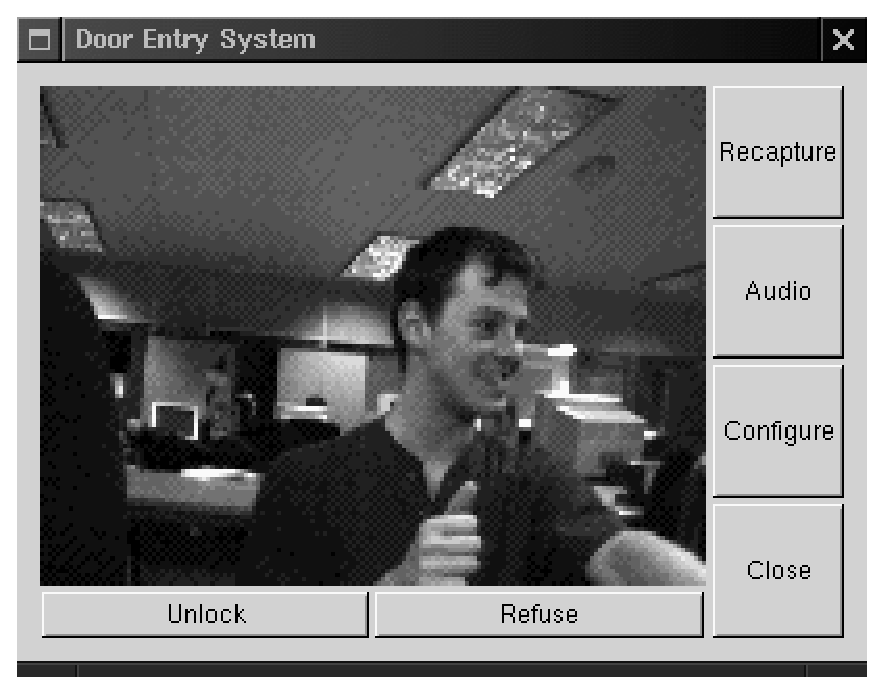
\includegraphics{gui_grab.ps}} \par}


\caption{\label{screenshot1}Screenshot of prototype GUI}
\end{figure}

The main window is shown in fig \ref{screenshot1}, page \pageref{screenshot1}.
If this window is minimised it will be activated whenever someone comes to the
door. Normally the video frames will be updated approximately once every second
and there will be no audio. When someone presses the buzzer and the PC user
reacts, two way sound transmission will begin and continue until a (long) timeout
expires, or the person is accepted or rejected. The functions of the various
buttons are as follows:

\begin{itemize}
\item recapture --- pressing this button transmits a request to the Motorola board
to recapture a frame of video;
\item unlock --- this causes the door to unlock;
\item refuse --- this denies entry;
\item audio --- this loads an audio configuration program (mixer);
\item config --- this opens the system configuration panel;
\item close --- this closes the interface window;
\item do not disturb (not present in the screenshot) --- this minimises the interface
window and tells the daemon not to pop it up.
\end{itemize}

\newpage
\section{Case Study: A school}


\subsection{Survey of local schools}

There are approximately six hundred schools in the Edinburgh area. We contacted
seven of them to get information about wether they would be interested and any
comments they had. The schools that were interested comments were

``They would prefer the system to only have video on the main entrance to the
school, but were worried that the school could be intimidating to pupils.''(Our
Lady of Lourdes RC Primary School)

``Unless the government made it a priority, then they would not be taking any
particular school precautions. The Cullen inquiries success in banning handguns
has taken away some of the fear from parents.''(North Queensferry Primary School)

``there would need to be strict tests on the system to make sure it did not
infringe pupil safety. They did consider the project a worthwhile exercise''
(Galashiels Academy)

Overall three of the schools contacted said that they would be interested in
a system for security, whilst four declared no interest for the time being.
If this survey is accurate then the market potential for the Edinburgh area
would be around 240 schools.


\subsection{The System}

Each entry point to the school will a reader and/or a keypad. The main entrance
to the school will be covered by the full system of a reader + keypad + camera.
All holders of the key will be able to enter through any control point. All
visitors will only be allowed to enter through the main entrance. Visitors have
to ring the buzzer to request entry. Communication can then take place to determine
the visitors identity. Dallas rings would be given to all the users of the school
and anyone else who is designated as needing one. This can include Councils
so that parts of the school can be rented out and used by community groups (the
scouts or sports clubs etc holders of the mechanical key should include all
three emergency services and a small number of the senior staff. 


\subsection{The Users}

The authorized users of the system will be the the staff and the pupils. The
staff will comprise of teachers, janitors, cleaners etc. Each user group will
have different demands on the times they will need to use the system.

\begin{itemize}
\item Teachers will need access at any time.
\item Cleaners may not start until the end of the school day.
\item Pupils should not be able to gain access outside school time. 
\item Visitors should only be able to enter through designated control points.
\end{itemize}
The system will be configurable, so that each user group can be given different
access rights. 


\subsection{The System Manager }

The system manager will have a system that is able to meet each users groups
need. They will be able to make changes to the database to control access times
and security levels. Pupils in year one of a primary school can not be expected
to remember long pin numbers or complicated routines. Therefore the first few
years in a primary school may have no PIN or a smaller PIN number than later
years. The response from schools was to not have PIN numbers at all for pupils
access but we should leave the option open.

The system manager should be the only one able to access the main computer.
This can be accomplished by utilizing existing iButton technology. Information
could be transferred between the iButton and a PC with a momentary contact.
Pressing the iButton to the Blue Dot Receptor, a \$15 (street price) \char`\"{}pipeline\char`\"{}
into the PC. The Blue Dot sticks to any convenient spot on the front of a PC
and is cabled to the serial or parallel port in the back. The information downloaded
would be a unique password to access the database. If the system manager is
the only one with the ring, he will be the only one who can access the database.


\subsection{SSERC questions}

How the system will react to the specific points mentioned in the interview
with Angus Morrison.

How does the system react if there is a fire alarm? 

\begin{quotation}
In the event of a fire the schools routine will not be affected by the sytem.
Each door can be manually opened from the inside to aid escape. 
\end{quotation}
How do you know when the system has stopped working? 

\begin{quotation}
When then the system stops working then the school will be unaffected as the
back up of a mechanical lock will allow the school to have the same security
level as at present. 
\end{quotation}
Can a pupil claim to be late because their Dallas ring failed to open the door? 

\begin{quotation}
By making the system durable (the Dallas rings have a life of around ten years)
pupils will not be able to get away with excuses. 
\end{quotation}
Does each door in the site have the system, and if they do, do they all come
with video cameras and are they all connected to the one PC? 

\begin{quotation}
Each door will require at least a reader but the system would be configurable
to any desired options. \emph{}
\end{quotation}
Most importantly, will this system still work for you in ten years? In twenty
years?''

\begin{quotation}
The system ideally should last as long as it is needed, if it is looked after
correctly.
\end{quotation}

\newpage
\section{Case Study: A Hospital}


\subsection{A survey of local hospitals}

There are approximately forty four hospitals in the Edinburgh area, we contacted
four of them to gauge there reaction to the system. In each case we talked to
someone in charge of the works department. Three of the four declaredan interest
in the product and there comments included

``Although the system would be successful in wards, it does seem as if it could
be be of more use in its automated format. We have specific areas of the hospital
that only certain people can enter, this includes the morgue, pharmacy and computer
departments. At present we use PIN numbers and keys to gain access but this
sounds like a more effective way of implementing our security strategy ''(Royal
Victoria Hospital)

``Any form of access contol to wards would have to be rigorously monitored
to ensure patient safety is not infringed''(Tippethill Hospital)

``If the system is reasonably cost effective then I can see it being of interest
to a lot of Hospitals''(Queen Margaret Hospital)


\subsection{The System}

At the entry point to a ward will be place the reader, keypad and the camera..
All holders of the key will be able to enter through the control point. All
visitors will only be allowed to enter by ringing ring the buzzer to request
entry. Communication can then take place to determine the visitors identity.
Dallas rings would be given to all the staff of the hospital who are deemed
to need one.

The second use would be the automated entry to points of security. These areas
include mortuary, pharmacy and medical cupboards etc Only the people who require
access to theses wards could be give access to them and the database of the
computer should be configurable so that information about peoples access rights
could be kept on record. Ideally each user will only need one dallas ring to
meet all their security needs. They will come to work unlock their door using
their dallas ring

\vspace{0.3cm}
{\centering \resizebox*{7cm}{5cm}{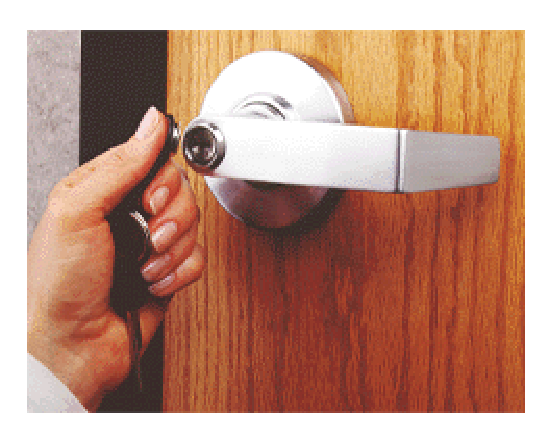
\includegraphics{../web/images/door3.ps}} \par}
\vspace{0.3cm}

They can then access their computer using a Blue Dot receptor. The technology
will kill off the need to have different security methods for different situations.
There wil be no need to remember all your keys, Pins and passwords, one technology
willl cover everything. Getting new security privalages will just be a matter
of updating the computer database, no need for waiting for a new key and no
need to ocme up with new passwords.


\subsection{The Users}

The authorized users of the system will be the the staff. The staff will comprise
of doctors nurses and porters etc etc. Each user group will have different demands
on the times they will need to use the system.

\begin{itemize}
\item Doctors will need instant access to wards, a delay in a call out for a cardiac
arrest could mean the difference between life and death.
\item Nurses would also require ease of access but may not need access to specific
areas of the hospital.
\item Visitors should be controlled from entering wards outside of visiting hours,
but during visiting hours there will probably need to have unlimited access
to patients.
\end{itemize}
The system will be configurable, so that each user group can be given different
access rights. 


\subsection{The System Manager }

The system manager will have a system that is able to meet each users groups
need. They will be able to make changes to the database to control access times
and security levels. Doctors should not need to learn PIN numbers but should
be able to gain access to areas with just their Dallas ring. The response from
hospitals was to not have PIN numbers at all to simplify matters, but again
we should leave the option open.

The system manager should be the only one able to access the main computer.
This can be accomplished by utilizing existing iButton technology. Information
could be transferred between the iButton and a PC with a momentary contact.
Pressing the iButton to the Blue Dot Receptor, a \$15 (street price) \char`\"{}pipeline\char`\"{}
into the PC. The Blue Dot sticks to any convenient spot on the front of a PC
and is cabled to the serial or parallel port in the back. The information downloaded
would be a unique password to access the database. If the system manager is
the only one with the ring, he will be the only one who can access the database.


\subsubsection{An interview with John Fitzpatrick (consultant anaethetist at the Southern
General.)}

Are you governed by any specific security mesures?

\begin{quotation}
``I have a security pass to identify myself, I have a password to access computer
systems, a key for my office and PIN and key number to access some chemical
cupboards.''
\end{quotation}
Would you benifit from having one device that could replace all of these?

\begin{quotation}
``I think anything that made life easier would be a good thing but it would
need to be as secure as present technology''
\end{quotation}

\newpage
\section{Manufacturing}


\newpage
\section{Competitors}

There are a great number of companies working in the field of security systems.
Most selling products that are scalable; if you want Access Control you buy
one part, if you need video as well then you add on an another component. A
minority of companies have designed specialized systems for residential or small
business' and only one or two have decided to target a unique market.


\subsection{School Security}


\subsubsection{ECr Concepts}

ECr Concepts in Merthyr Tydfil plan to introduce a new credit card-style pass
system to secondary and primary schools. It will monitor on computer everything
from attendance to what children eat for lunch. Parents can pay for school meals
in advance and this will be recorded on a computer. When a child goes for a
meal, the card is swiped and a picture of the youngster appears on the computer
for identification. What is ordered is also recorded.

Parents can ask for a weekly read-out of meals eaten and obtain a breakdown
of their fat, carbohydrate and protein content to ensure a healthy, balanced
diet. The card will incorporate an entry function. It can be used to enter the
school and selected controlled areas. As well as keeping out intruders, staff
will be able to monitor attendance and record daily movements in the school.

Their local councillor stated: 

\begin{quotation}
``It sounds a great idea for the future of security and paying for meals and
other services in schools. The card will not only ensure that unauthorized access
is not allowed at school but can cover simple everyday things like ensuring
children have their school meals. \emph{}I can envisage a day in the not too
distant future when every schoolchild in Britain will have one of these cards
to use in their schools.\char`\"{}
\end{quotation}

\subsection{Specialized Security Systems}


\subsubsection{CEM Security Systems}

CEM security systems has a similar marketing strategy to our own. They have
seen a specific gap in the market (airport security) and designed their product
accordingly. 

Since installing their first system at Belfast International Airport in 1987,
CEM Systems Ltd. has migrated their Airport 2000 system throughout the major
airports of the United Kingdom including Heathrow, Gatwick, Stansted, Glasgow,
Manchester, East Midlands, Luton and Edinburgh. CEM have also installed similar
systems in airports around the globe. 

Each different airport in the United Kingdom has differing security needs. However,
all use the Airport 2000 Visual Imaging Pass Production System (VIPPS) in one
manner or another. VIPPS captures, compresses, stores and retrieves graphical
and textual data such as images, logos and signatures. 

Their chairman states:

\begin{quotation}
\char`\"{}VIPPS allows the airport to add graphical and textual information
to the database, capture images from live or still cameras and photographs,
retrieve and update previously entered data, write data to various card technologies
and define badge layouts.\char`\"{}
\end{quotation}

\subsection{Security using iButton technology}


\subsubsection{Seadan Security \& Electronics}

Seadan Security \& Electronics offers the EL1200 Access System for physical
access control of medium-size offices and buildings, or areas within buildings.
The EL1200 system can store information for up to 1,500 individuals permitted
to access a building. 

To gain entrance to a building secured with the EL1200 Access System, an employee
touches his or her iButton-based key ring or token to an iButton reader mounted
by the door, then enters their Personal Identification Number (PIN). The system
compares the data read from the iButton and PIN number to the system's data
base, then unlocks the door if the data is verified as correct. An entry log
is maintained by the EL1200 showing all persons who entered by a specific door,
and what date and time they entered. 

The system allows for 10 access time zones or categories, allowing the system
to compensate for a company's holiday schedule. The iButton reader unit has
12 keys and 4 display characters for simple operation and programming. Output
point can be configured as a door open alarm output, timer-driven output, or
sensor alarm output Standard software packages are available 

The EL1200 is equipped with a standard interface for network operation. Ultimately
connecting the units to a PC for centralized monitoring and control. 


\subsubsection{Cansec Systems Ltd. }

Cansec offers two iButton access readers for use with Cansec- and OEM-manufactured
access control systems, and the associated TAS100 Data Management Software package
supports up to 1,000 users and four reader groups for either the TAS100 or the
RT100. 

TAS100 Touch Access Stand-Alone System is a self-contained, programmable access
control system. It is simple to install and operate, requiring no communications
wires for use. The system includes easy-to-use programming software, and access
keys are programmed with a read/write iButton key. The reader features rugged
metal construction and bi-color LED status. A Sonalert tone alerts users to
someone attempting or achieving access to a building or room. . A bi-colored
LED and Sonalert provide users with both visual and audible signals of access
being granted or denied. The face plate and stainless steel read head are vandal-resistant
and suitable for both indoor and outdoor use. While in use, the last 64 access
granted messages can be retrieved from the Reader with an audit key.


\subsection{General Security Companies}


\subsubsection{Gyr secutity }

Gyr market an advanced security management system specifically designed to assist
professional facilities and security managers by providing a single screen solution.
It's claimed to be the ideal tool for building access, parking access and CCTV
control at single or multiple locations.


\subsubsection{PAC access control}

PAC for Windows Residential is a PC based housing security system running under
Microsoft Windows. The system has been designed for single and multi-block estates
with up to 30,640 doors and any number of users.

PAC for Windows Residential offers a wide range of building management functions
which include: monitoring and controlling security cameras; linking to paging
systems for mobile personnel and monitoring fire doors and lift doors to check
wether they have been left open.

Tenants are issued with PAC proximity keys, three per flat, color coded for
easy recognition. Local authority staff carry PAC proximity ID cards which include
a photograph for identification purpose

At the Housing Office, PAC readers are fitted to external doors, to restrict
access to the building, and system administration is carried out at a central
PC. Additional PCs are located in the concierge of each of the residential blocks
for monitoring alarms and system events, and to allow guards manual control
of doors and carpark barriers.

Ancillary equipment, including panic buttons, fire exits, ventilation and heating
equipment in the main building are monitored using PAC Alarm Event Managers.
Concierge and maintenance staff are alerted to problems via pagers.

Car park lighting is time-controlled via the PAC Alarm Event Manager.

Elevator control is used in each of the residential blocks to restrict access
by tenants to different floors of the main building.


\subsection{Conclusion}

There are only a couple of companies working in the field of iButton building
access control, none of which have identified a niche market or offer audio
visual communication. 

Our Group is unique in that it is supplying a state of the art system that will
meet the needs of our market. Like Cemsys we have identified a specific need
and therefore we should be able to reap the dividend.


\newpage
\section{Appendix}


\subsection{Serial ID Button}

What is an iButton? 

\vspace{0.3cm}
{\centering 
\includegraphics{../web/images/ibutton.ps} \par}
\vspace{0.3cm}

The iButton is a 16mm computer chip housed in a stainless steel can. The iButton
can be worn by a person or attached to an object for up-to-date information
at the point of use.The steel button is rugged enough to withstand harsh outdoor
environments; it is durable enough for a person to wear everyday on a digital
accessory like a ring, key fob, wallet, watch, or badge.

\vspace{0.3cm}
{\centering 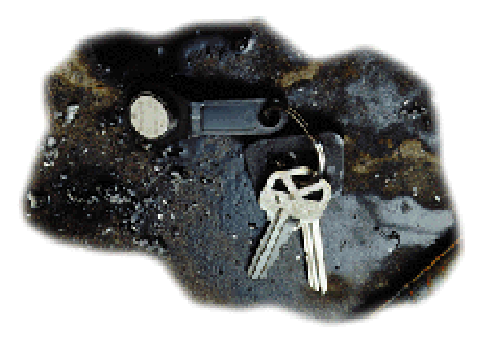
\includegraphics{../web/images/overvw3.ps} \par}
\vspace{0.3cm}

There are a variety of buttons with different features. Each starts with a guaranteed-unique
registration number engraved in the silicon. Some buttons add computer memory
to store typed text or digitized photos; information can be updated as often
as needed with a simple, momentary contact. Other buttons contain a real-time
clock to track the number of hours a system is turned on for maintenance and
warranty purposes; a temperature sensor for applications where spoilage is a
concern, such as food transport; a transaction counter that allows the button
to be used as a small change purse; or complete cryptographic circuitry to secure
Internet transactions.  

The fragile silicon chip within the iButton is protected by stainless steel.
You can drop it, step on it, scratch it, or wear it swimming. iButtons have
a useful life of around 10 years while a magnetic / barcode system 's useful
life is only 3 months to 2 years depends on the usage and maintenance. The ibutton
has a unique Read Only Serial Number, no one can copy your ibutton or master
ibutton.

Authorization Buttons are sophisticated microelectronics, sealed into miniature
stainless steel cans, creating a low cost, portable medium for storing and controlling
access to sensitive information

The iButton is ideal for any application where information needs to travel with
a person or object. An iButton can grant its owner access to a building, a PC,
a piece of equipment, or a vehicle. Attached to a work tote, it can measure
a variety of processes to improve efficiency, such as manufacturing, delivery,
and maintenance. Some versions of the iButton can be used to store cash for
small transactions, such as transit systems, parking lots, and vending machines.
The iButton can also be used as an electronic asset tag to store information
needed to keep track of valuable capital equipment. 

Users of the iButtons include the U.S. Post Office, which has iButtons affixed
to blue corner mailboxes nationwide so they can do the tracking needed to ensure
on-time delivery of the mail. Ryder has its entire truck fleet fitted with iButtons
that track vehicle maintenance. Citizens of Istanbul, Turkey store digital cash
in the iButton, using the device as a small change purse on their mass transit
system. 

iButton technology works well in commercial applications where multiple users
and continuous use put stress on less robust electronic devices. In hotels,
for instance, children cannot stick paper into the iButtons door receptors,
and the iButton never jams in a lock. The usage instructions are superbly simple
and quickly demonstrable: just press the button to the receptor. Besides being
durable, reliable and easy to use, iButton technology also wins management approval
because it consumes virtually zero power. In large facilities such as hospital,
office, and apartment buildings, low maintenance and power consumption are factors
that register on the black side of the ledger. 

In conclusion, the architecture is very elegant, can migrate into the mainstream
PC market with little engineering effort, and offers opportunity for the emergence
of distributed security solutions that are both cost effective and reliable. 


\subsection{Blue Dot Receptor }

\vspace{0.3cm}
{\centering 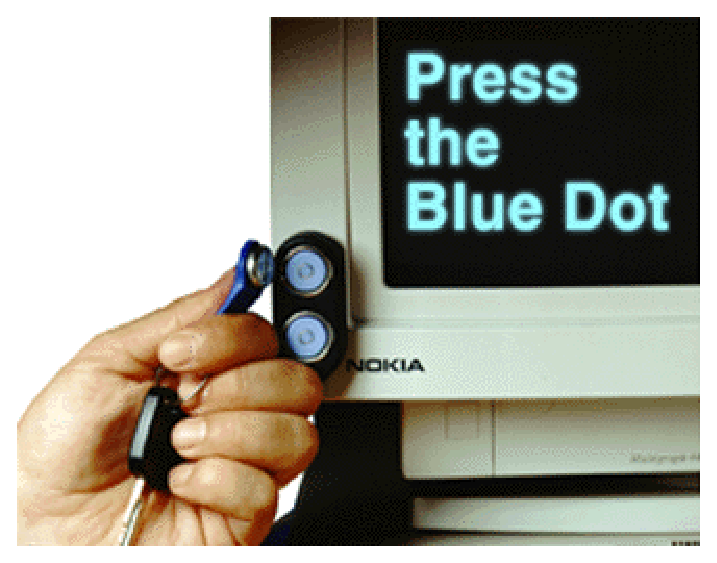
\includegraphics{../web/images/blue.ps} \par}
\vspace{0.3cm}

The DS1402 Blue Dot Receptor is used to make iButton access convenient. The
cable is connected to either the DS1410E or DS1411. The Blue Dot can be mounted
anywhere in the desktop area that is convenient. 

Communication between the iButton and the host is accomplished by simply pressing
the iButton to the Blue Dot. One method is to touch the iButton to the Blue
Dot momentarily. If the iButton is pushed further into the Blue Dot, it will
snap in and dwell, allowing hands-free operation. 

Two Blue Dots are provided to accommodate instances where multiple iButtons
are required to complete a transaction. For example, a company's policy may
be to require both an employee and a supervisor to authenticate access to sensitive
information stored on a network server. Operation modes can also be interchanged
arbitrarily (i.e., the employee's iButton may be required to dwell and the supervisor's
iButton need only make momentary contact). 


\newpage
\section{Bibliography}

\emph{Building Security: Are You Overlooking Something?} by Robert Hager, IDenticard
Systems, Inc. 

www.telegraph.co.uk

www.cemsys-na.com

www.gyr.com

www.pac.co.uk 

www.ibutton.com/Connections/Catalogs/seadan.html

Thanks to

The Royal Victoria Hospital

The Victoria Hospital

The Queen Margaret Hospital

Tippethill Hospital

Our Lady of Lourdes RC Primary

North Queensferry Primary

Swinton Primary

Firhill High

Galashiels Academy

Inverkeithing High

Mr N Macleod

Mr B Liddle

Mr A Morrison

\end{document}
